\subsubsection{Environment}

\begin{figure}[H]
\centering
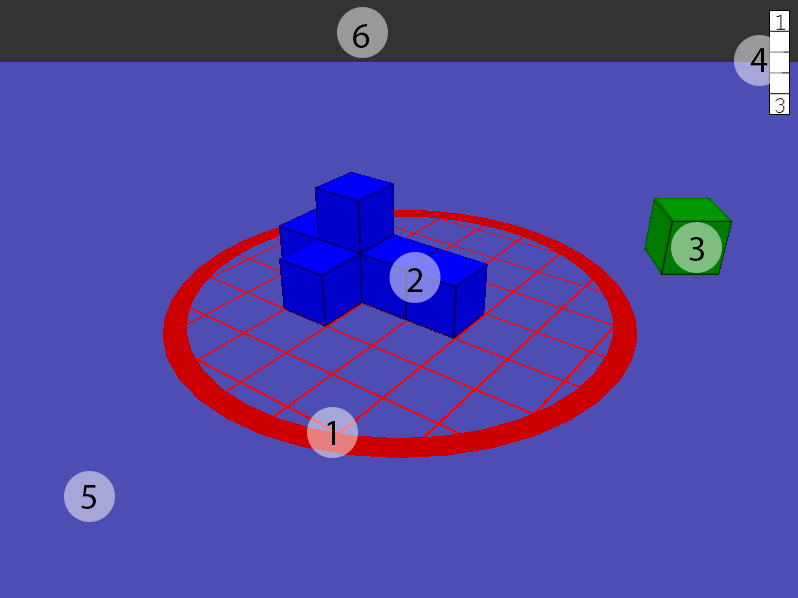
\includegraphics[width=\textwidth]{env_comps}
\caption{\label{fig:environmentcomps} Common rendering of the task environment. Visual elements: 1-Circular~grid 2-Building~blocks 3-Creation~block 4-Target~indicator 5-Floor 6-Horizon}
\end{figure}

\noindent The task environment is a virtual graphical computer program for building virtual block structures using either a Leap Motion or keyboard and mouse. Figure~\ref{fig:environmentcomps} shows a common rendering from the task environment in which all visual elements have been labeled. In the center of the screen users are presented with a circular grid that is segmented into several squares, effectively representing a grid with an circular border. On this grid building blocks can be positioned, either directly on the grid or stacked on top of other building blocks. New building blocks can be obtained by interacting (clicking with the mouse or grabbing with the Leap Motion) with the creation block just next to the circular grid. The target indicator on the top right corner gives the user a representation of the block structure that should be created on the grid before the user can move further.

\paragraph{Circular grid}
The circular grid is made out of square grid-cells and a limit circle which has a radius that is slightly bigger than $3.5$ grid-cells width. The grid is able to rotate $360^{\circ}$ around the y-axis of the center of this grid (the origin). In resting state the grid and limit circle have a red color, but while the circle is rotated by the user the limit circle temporarily becomes orange until it reaches resting state once more. 

\paragraph{Building blocks}
The building blocks are 3D cubes with dimensions corresponding to $1\times 1\times 1$ the width of a grid-cell and all have black outline at the edges. Building blocks can be lifted, dragged around, and dropped by the user. While building blocks are lifted they cast a shadow directly below them in order to know their position relative to the grid. In resting state the building blocks are blue, when they are being dragged they are orange and when a user points at them and does not drag anything they become light-blue. 

\paragraph{Creation block}
The creation block has the same dimensions as the building blocks, but has a different color. A user can use the creation block to obtain new building blocks by interacting with it. When a user points at the creation block it lights up light-green, otherwise it has a dark-green color. In the version of the environment used for the experiment the creation block was positioned one grid-cell width above the floor level to compensate for the limited vertical detection range of the LEAP Motion.

\paragraph{Target indicator}
The target indicator is a 2D image always visible to the user. It shows the currently active target structure (or goal) that should be created by the user with the building blocks in order to advance to the next task and to complete the experiment. The image is always shown in a single orientation, but actual task completion can be achieved by creating a $90^{\circ}$, $180^{\circ}$ or $270^{\circ}$ degree rotated version of the target structure within the grid as well. Also it does not matter where in the grid the solution is created.

\paragraph{Floor}
The floor is merely a plane that indicates the lower limit of where building blocks can be positioned. It also serves as a surface to show the shadows from the building blocks on.

\paragraph{Horizon}
A small strip of horizon is made visible to help the user understand the orientation when tilting the camera up and down. The current color of the horizon is dark-gray.



\paragraph{Design rationale}
The program was developed with the use of jMonkeyEngine, an open source 3D game engine written in Java. For development we used the Software Development Kit that comes with the engine, which provides a high level interface for numerous 3D functions and data-structures (e.g. spatial manipulation, quaternions and 3D meshes) and also provides a high degree of control for developers by being completely compatible with the Java programming language. 

Both the User Interface (UI) and the user interactions were designed to be minimalistic, simple and intuitive in order to prevent users having to learn a lot before they could use the system. 
